\documentclass[compress]{beamer}
\usetheme{sthlm}

%-=-=-=-=-=-=-=-=-=-=-=-=-=-=-=-=-=-=-=-=-=-=-=-=
%        LOADING BEAMER PACKAGES
%-=-=-=-=-=-=-=-=-=-=-=-=-=-=-=-=-=-=-=-=-=-=-=-=

\usepackage{
booktabs,
datetime,
dtk-logos,
graphicx,
multicol,
pgfplots,
ragged2e,
tabularx,
tikz,
wasysym,
multirow,
float,
caption,
subcaption
}

\pgfplotsset{compat=1.8}

\usepackage[utf8]{inputenc}
\usepackage[portuguese]{babel}
\usepackage[T1]{fontenc}
\usepackage{newpxtext,newpxmath}
\usepackage{listings}

\lstset{ %
language=[LaTeX]TeX,
basicstyle=\normalsize\ttfamily,
keywordstyle=,
numbers=left,
numberstyle=\tiny\ttfamily,
stepnumber=1,
showspaces=false,
showstringspaces=false,
showtabs=false,
breaklines=true,
frame=tb,
framerule=0.5pt,
tabsize=4,
framexleftmargin=0.5em,
framexrightmargin=0.5em,
xleftmargin=0.5em,
xrightmargin=0.5em
}



%-=-=-=-=-=-=-=-=-=-=-=-=-=-=-=-=-=-=-=-=-=-=-=-=
%        LOADING TIKZ LIBRARIES
%-=-=-=-=-=-=-=-=-=-=-=-=-=-=-=-=-=-=-=-=-=-=-=-=

\usetikzlibrary{
backgrounds,
mindmap
}

%-=-=-=-=-=-=-=-=-=-=-=-=-=-=-=-=-=-=-=-=-=-=-=-=
%        BEAMER OPTIONS
%-=-=-=-=-=-=-=-=-=-=-=-=-=-=-=-=-=-=-=-=-=-=-=-=

\setbeameroption{show notes}

%-=-=-=-=-=-=-=-=-=-=-=-=-=-=-=-=-=-=-=-=-=-=-=-=
%        BEAMER COMMANDS
%-=-=-=-=-=-=-=-=-=-=-=-=-=-=-=-=-=-=-=-=-=-=-=-=


%-=-=-=-=-=-=-=-=-=-=-=-=-=-=-=-=-=-=-=-=-=-=-=-=
%
%	PRESENTATION INFORMATION
%
%-=-=-=-=-=-=-=-=-=-=-=-=-=-=-=-=-=-=-=-=-=-=-=-=

\title{Consistência de dados}
\subtitle{DCE540 - Computação Paralela e Distribuída}
%\date{\small{\jobname}}
\author{\texttt{Iago Carvalho}}
\institute{\texttt{Departamento de Ciência da Computação}}

\hypersetup{
pdfauthor = {Iago A. Carvalho},      
pdfsubject = {Computação Paralela e Distribuída},
pdfkeywords = {},  
pdfmoddate= {D:\pdfdate},          
pdfcreator = {WriteLaTeX}
}

\begin{document}

\begin{frame}
\titlepage

\end{frame}

%% --------------------------------------------------------

\begin{frame}{Consistência e replicação de dados}

É muito comum utilizarmos replicação de dados
\begin{itemize}
    \item Melhorar performance do sistema
    \item Realizar cópias de segurança de dados
\end{itemize}

\vspace{0.5cm}

Quando existem dados replicados, cria-se um novo problema
\begin{itemize}
    \item Consistência de dados
    \item Caso um dado seja alterado, todas as cópias devem ser atualizadas
\end{itemize}

\vspace{0.5cm}

Este é um problema relativamente grave quando temos diversos componentes querendo acessar e alterar um mesmo dado de forma simultânea
\end{frame}

%% --------------------------------------------------------

\begin{frame}{Razões para replicação}

\begin{enumerate}
    \item Tolerância a falhas e segurança
    \begin{itemize}
        \item Caso o servidor que contém uma cópia falhe, é possível simplesmente migrar para outro
        \item Caso um servidor esteja muito congestinado, pode-se utilizar outro
        \item Segurança contra dados corrompidos
    \end{itemize}
    \vspace{0.5cm}
    \item Performance do sistema distribuído
    \begin{itemize}
        \item Sistemas distribuídos tem que ser escaláveis
        \item Em sistemas de grande porte (nível nacional ou internacional), é importante termos os dados sempre próximos (fisicamente) dos usuários
        \item Balanceamento de carga
    \end{itemize}
\end{enumerate}

\end{frame}

%% --------------------------------------------------------

\begin{frame}{Consistência de dados}

Quanto estamos trabalhando com consistência de dados, devemos levar em consideração duas coisas

\vspace{0.5cm}

\begin{enumerate}
    \item Atual implementação da consistência
    \begin{itemize}
        \item Como os dados estão distribuídos
        \item Em que localização (física) eles estão
        \item O acesso aos dados é rápido e efetivo?
    \end{itemize}
    \vspace{0.5cm}
    \item Como manter os dados consistentes
    \begin{itemize}
        \item Consistência forte
        \item Cache
        \item Algoritmos de atualização de dados
    \end{itemize}
\end{enumerate}
\end{frame}

%% --------------------------------------------------------

\begin{frame}{Replicação como técnica de escalonamento}

A principal idéia é replicar os dados em lugares geograficamente diferentes
\begin{itemize}
    \item Distribuídos fisicamente através dos locais onde um sistema distribuído é utilizado
    \item Esta distribuição leva em conta dois aspectos
    \begin{enumerate}
        \item Número de usuários em um determinado local
        \item Distância dos usuários até o local
    \end{enumerate}
\end{itemize}

\vspace{0.5cm}

Entretanto, esta replicação pode levar a inconsistência
\begin{itemize}
    \item Mesmo que não exista inconsistência, também deve-se considerar o maior tráfego de rede necessário para atualizar todos os arquivos
\end{itemize}
\end{frame}

%% --------------------------------------------------------

\begin{frame}{Mau uso de replicação}

Considere uma aplicação $P$ qualquer
\begin{itemize}
    \item Ela acessa um dado replicado $N$ vezes por minuto
\end{itemize}

\vspace{1cm}

O dado é completamente atualizado $M$ vezes por minuto
\begin{itemize}
    \item $N <\!\!< M$
\end{itemize}

\vspace{1cm}

Tráfego desnecessário na rede
\begin{itemize}
    \item Principalmente se o arquivo replicado for grande
\end{itemize}
\end{frame}

%% --------------------------------------------------------

\begin{frame}{Tipos de consistência de dados}

Consistência apertada (replicação síncrona)
\begin{itemize}
    \item Dados só são ditos serem replicados quando realmente são iguais
    \item Desta forma, é necessário mante-los sempre atualizados
    \item Atualização é muito cara
\end{itemize}

\vspace{0.5cm}

Consistência frouxa (replicação assíncrona)
\begin{itemize}
    \item Dado é atualizado somente onde é realizada a operação
    \item \textit{Clock} é salvo e enviado para as réplicas
    \item Caso alguém tente acessar uma réplica, o dado é então atualizado
\end{itemize}

\end{frame}

%% --------------------------------------------------------

\begin{frame}{Modelos de consistência centrado em dados}

Um modelo de consistência é basicamente um acordo entre os processos
\begin{itemize}
    \item Todos eles concordam com um conjunto de regras
    \item Todo processo de atualização de dados deve seguir as regras acordadas
    \item Modelos de consistência são implementados pelo \textit{middleware} de um sistema distribuído
\end{itemize}

Modelos de consistência centrado em dados
\begin{itemize}
    \item Classifica operações como 
    \begin{itemize}
        \item Leitura
        \item Escrita
    \end{itemize}
    \item Operações de escrita tem que ser propagadas para as réplicas dos dados
\end{itemize}
\end{frame}

%% --------------------------------------------------------

\begin{frame}{Consistência contínua}

Refere-se ao \textit{quanto} de inconsistência um sistema distribuido pode tolerar
\begin{itemize}
    \item Uma linha de código
    \item 5\% do banco de dados alterado
    \item Duas atualizações do repositório
    \item Três horas de diferença
    \item $\ldots$
\end{itemize}

\vspace{0.5cm}

Ao atingir este limite, o sistema distribuído deve então atualizar todas as réplicas dos dados

\end{frame}

%% --------------------------------------------------------

\begin{frame}{Unidade de consistência}

Conit (do inglês \textit{consistency unit})
\begin{itemize}
    \item Representa a unidade sobre a qual consistência defe ser aferida
\end{itemize}

\vspace{0.5cm}

No nosso caso, a consistência normalmente é um único dado
\begin{itemize}
    \item Uma entrada em um banco de dados
    \item Um arquivo de código-fonte
    \item Uma atualização de um repositório
\end{itemize}
\end{frame}

%% --------------------------------------------------------

\begin{frame}{Consistência sequencial}

O resultado de qualquer execução é a mesma se as operações de todos os processos sob o conjunto de dados são executadas em uma ordem sequencial

\vspace{1cm}

\centering 

Sequencial \hspace{4cm} Não sequencial

\vspace{.15cm}

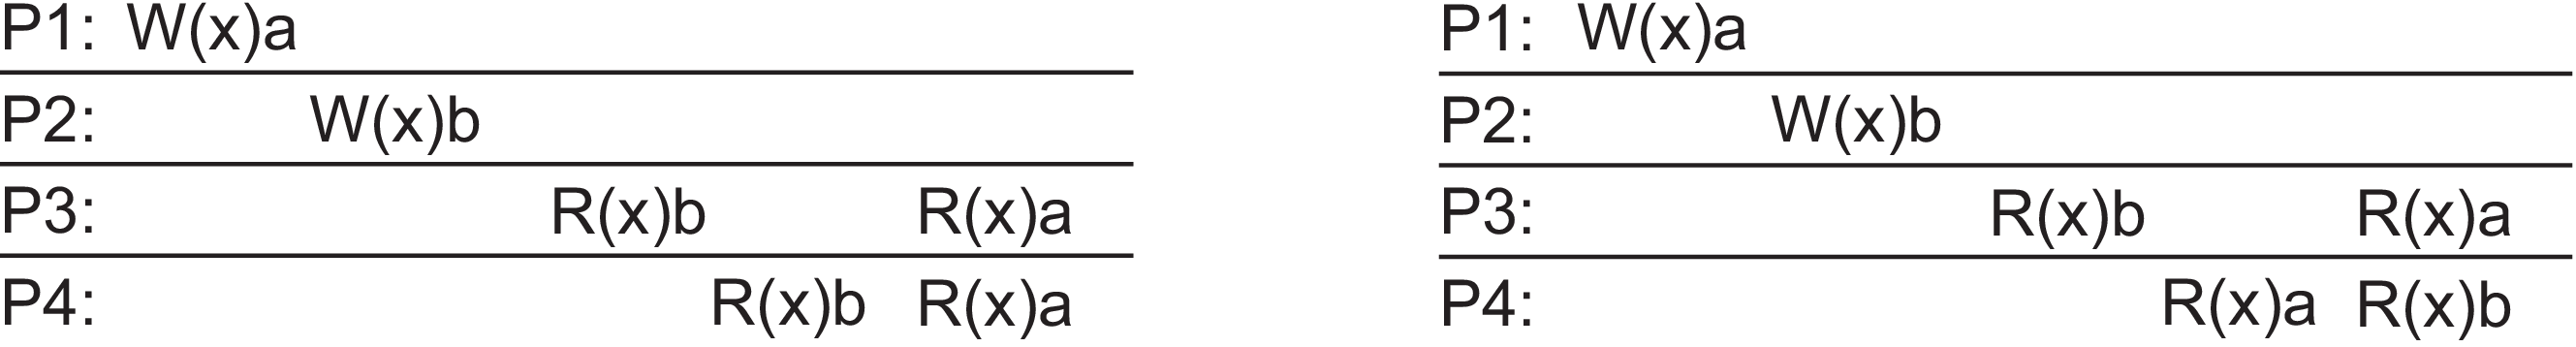
\includegraphics[width=\textwidth]{images/sequencial.png}
\end{frame}

%% --------------------------------------------------------

\begin{frame}{Consistência casual}

Operações de escrita concorrentes podem ser vistas em diferentes ordens por cada processo
\begin{itemize}
    \item Relaxamento da consistência sequencial
\end{itemize}

\vspace{0.5cm}

Considere $W(x)b$ e $W(x)c$ como concorrentes

\vspace{1cm}

\centering 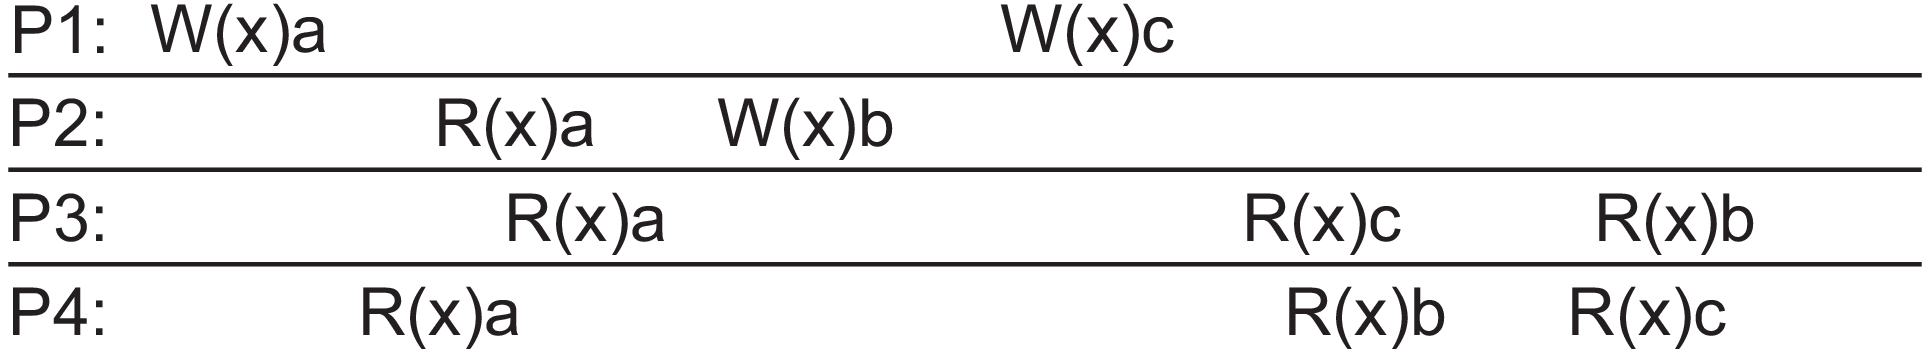
\includegraphics[width=\textwidth]{images/casual.png}
\end{frame}

%% --------------------------------------------------------

\begin{frame}{Sessão crítica e consistência}

Usa operações de \textit{lock} ($L(x)$) e \textit{unlock} ($U(x)$)

\vspace{1cm}

\centering 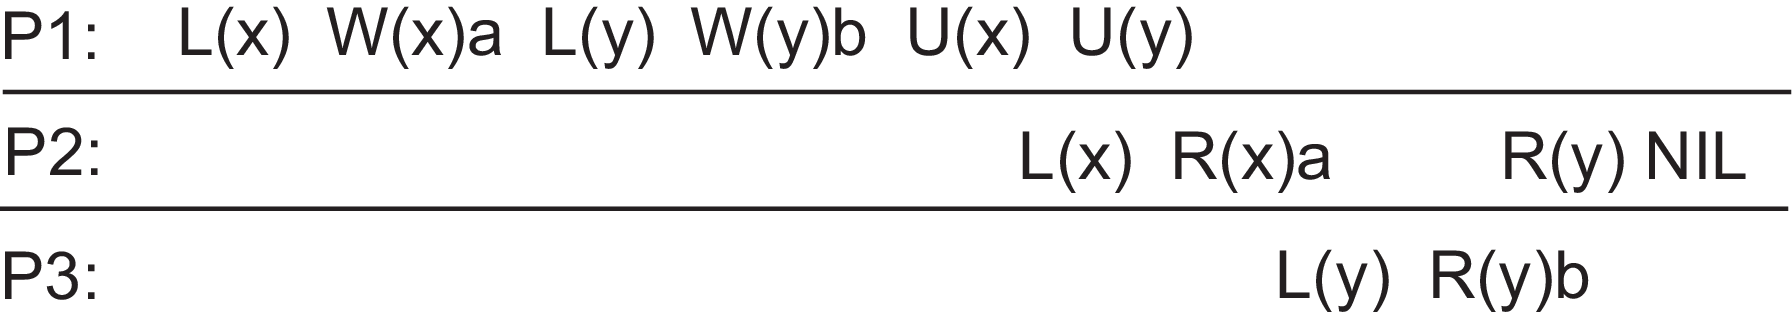
\includegraphics[width=\textwidth]{images/lock.png}
\end{frame}

\end{document}
